\subsection{Long Short Term Memory}
\label{sec:LSTM}

Die einzige bisher vorgestellte Architektur von \acrshortpl{nn} ist das Feedforward-Netz.
Diese Netzarchitektur eignet sich gut für Klassifizierungsaufgaben.
Die vorliegende Arbeit beschäftigt sich jedoch mit Standorten von mobilen Radarkontrollen über die Zeit, also mit sequenziellen Daten.
Feedforward-Netze können zeitliche Zusammenhänge nicht darstellen und nicht erlernen, da sie keinen internen Zustand haben.
Das bedeutet, dass die Ausgabe des \acrshort{nn}s nur abhängig von der aktuellen Eingabe ist, nicht aber von vorherigen Eingaben.

Abhilfe hierbei bieten \k{rekurrente neuronale Netze} (\acrshortpl{rnn}).
Wie Chollet in \cite[S. 252]{DeepLearningPythonKeras} erläutert, besitzen rekurrente \acrshortpl{nn} einen internen Zustand, der alle bisherigen Eingaben repräsentiert.
Eine Ausgabe ist dann sowohl von der Eingabe als auch vom internen Zustand abhängig.
Implementiert wird dieses Verhalten durch eine Schleife im \acrshort{nn}.
In \autoref{fig:RNNSchleife} ist diese Architektur schematisch dargestellt.

\begin{figure}[h]
    \centering
    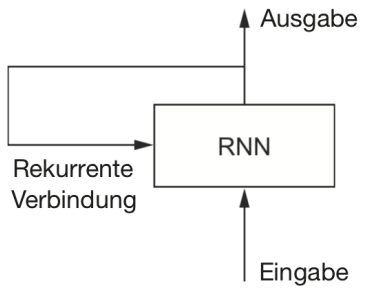
\includegraphics[width=0.5\textwidth,height=4cm,keepaspectratio=true]{content/images/RNNSchleife.png}
    \caption{Schleife in einem \acrshort{rnn} \cite[Abb. 6.9]{DeepLearningPythonKeras}}
    \label{fig:RNNSchleife}
\end{figure}

Ein einfaches \acrshort{rnn} berechnet die Ausgabe $Y_t$ nach \cite[S. 253]{DeepLearningPythonKeras} wie in \autoref{eq:RNN} gezeigt.

\begin{equation}
    Y_t = a(W \cdot X_t + U \cdot S_t + b)
\label{eq:RNN}
\end{equation}

Dabei steht $X_t$ für die Eingabe und $S_t$ für den internen Zustand, jeweils zum Zeitschritt $t$.
$W$ und $U$ sind Matrizen, die die trainierbaren Gewichtungen enthalten und $b$ ist ein trainierbarer Bias-Vektor.
Nach der Berechnung wird die Ausgabe zum neuen internen Zustand, man könnte also $S_t$ in \autoref{eq:RNN} durch $Y_{t-1}$ ersetzen.

Diese einfache Architektur unterliegt nach \cite[S. 260]{DeepLearningPythonKeras} jedoch dem sogenannten \emph{Problem des verschwindenden Gradienten}.
Dieser Effekt sorgt dafür, dass relativ weit zurückliegende Eingaben praktisch keinen Einfluss mehr auf die Ausgabe haben.
Es sind jedoch Anwendungsfälle denkbar, in denen auch weiter zurückliegende Ereignisse einen großen Einfluss auf die Gegenwart haben.
Für die Vorhersage von mobilen Radarkontrollen könnte beispielsweise von Bedeutung sein, wie die Verteilung der Radarkontrollen vor 15 Tagen ausgesehen hat.
Das liegt daran, dass die Daten eine Periodizität von z.B. 15 Tagen aufweisen könnten.

Zur Lösung dieses Problems gibt es verschiedene alternative \acrshort{rnn}-Architekturen.
Eine davon ist \acrfull{lstm}.
Wie der Name vermuten lässt, ermöglicht die \acrshort{lstm}-Architektur, sowohl Abhängigkeiten von weit zurückliegenden als auch aktuellere Eingaben zu lernen.
Die \acrshort{lstm}-Architektur ist in \autoref{fig:LSTMCell} dargestellt.

\begin{figure}[h]
    \centering
    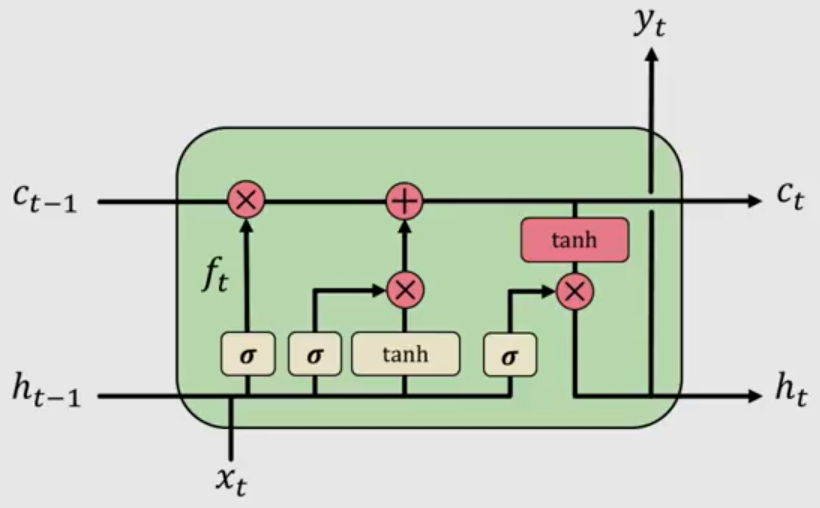
\includegraphics[width=0.8\textwidth,height=6cm,keepaspectratio=true]{content/images/LSTMCell.png}
    \caption{Schematische Darstellung einer \acrshort{lstm}-Zelle \cite{6S191RNN}}
    \label{fig:LSTMCell}
\end{figure}

Eine \acrshort{lstm}-Zelle enthält drei sogenannte Tore (engl. Gates).
Ein Tor ist selbst ein \acrshort{nn}.
Die drei Tore und ihre jeweilige vorgesehene Wirkung sind nach \cite{6S191RNN}:

\begin{enumerate}
    \setlength\itemsep{0.2em}
    \item \textbf{Vergessens-Tor}: Dieses Tor sorgt dafür, dass irrelevante Informationen aus dem vorherigen Zustand "`vergessen"' werden.
    \item \textbf{Merk-Tor}: Dieses Tor fügt dem Zustand relevante neue Informationen hinzu.
    \item \textbf{Ausgangs-Tor}: Dieses Tor bestimmt, welche Informationen aus dem Zustand zum Ausgang der Zelle gelangen sollen.
\end{enumerate}

Amini und Soleimany stellen die vorgesehene Wirkung der Tore in \cite{6S191RNN} ohne weitere kritische Auseinandersetzung dar.
Wie Chollet in \cite[S. 263]{DeepLearningPythonKeras} argumentiert, ist diese Wirkung jedoch keinesfalls garantiert.
Die tatsächliche Wirkung hinge nach Chollet viel mehr von den letzendlich antrainierten Gewichtungen der Tore ab.
Amini und Soleimany sind sich jedoch mit Chollet einig, dass es nicht wichtig ist, die interne Funktionsweise einer \acrshort{lstm}-Zelle im Detail zu verstehen.
Chollet geht noch einen Schritt weiter und argumentiert, dass dies ganz allgemein keine Aufgabe der Menschen sei.
Wichtig ist nach Chollet, Amini und Soleimany nur sich im klaren zu sein, welche Aufgabe eine \acrshort{lstm}-Zelle erfüllt - sie ermöglicht es, sowohl langfristige als auch kurzfristige Zusammenhänge anhand der Trainingsdaten zu erlernen.
